% !TEX root = ../master.tex

\section{Running Examples}\label{examples:sec}
Based on the previous descriptions, we have created two examples which will work as IoT use-cases, and will be the base for our following discussions and implementation.
These examples contain only constructions supported by our implementation.
Attached to each example is also a graph, visualizing the program information flow, with the following legend:
\begin{figure}[H]
  \centering
  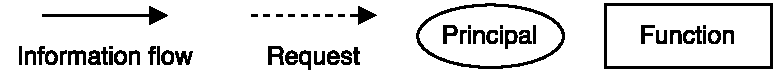
\includegraphics[scale=0.8]{figures/dlm_legend}
  \caption{Information flow graph legend}
  \label{example:legend}
\end{figure}
The two shapes \emph{channel} and \emph{time handler} will be relevant later in the report, when we start introducing more concepts.
In the graphs we also have to abstractions that are not apparent when looking at the code examples.
The main function has been left out, and the \emph{request} flows represent calls to the program, through some means (e.g. a call from another program or through a web-request).
In the code examples themselves, the logic in the main function will also not completely represent an actual implementation, as we have abstracted away from how the program will actually be run or called.

\subsection{Smart meter bill calculation}
Related to the protection of smart meter data, we have created a simple example (see \cref{example:code:calculate_bill} and \cref{example:graph:calculate_bill}) which uses data from both consumer and electrical company in order to calculate a bill.
Here we make use of 4 auxiliary functions: \dlmc{get_latest_usage}, \dlmc{get_latest_prices}, \dlmc{send_to_consumer}, and \dlmc{send_to_electrical_company}, which represent ways of either obtaining data from outside the program, or sending data to outside of the program.

\begin{lstlisting}[float, style=dlmc, numbers=left, caption={Smart meter bill calculation example}, label=example:code:calculate_bill]
typedef struct usage {
  int start_time;
  int usage_in_Wh;
} usage;

typedef struct price {
  int start_time;
  int price_in_cents;
} price;

usage *get_latest_usage();
price *get_latest_prices();
void send_to_consumer(int bill);
void send_to_electrical_company(int bill);

int calculate_bill() {
  int usage_count = 100;
  int prices_count = 100;
  usage *latest_usage = get_latest_usage();
  price *latest_prices = get_latest_prices();
  int result = 0;

  int i = 0;
  int j = 0;
  while (i < usage_count) {
    while ((j < prices_count-1) &&
        (latest_prices[j+1].start_time <= latest_usage[i].start_time)) {
      j = j + 1;
    }
    result = result + latest_usage[i].usage_in_Wh *
      latest_prices[j].price_in_cents;
    i = i + 1;
  }
  return result;
}

int main(int argc, char **argv) {
  int bill = calculate_bill();
  send_to_consumer(bill);
  send_to_electrical_company(bill);
}
\end{lstlisting}

\begin{figure}
  \centering
  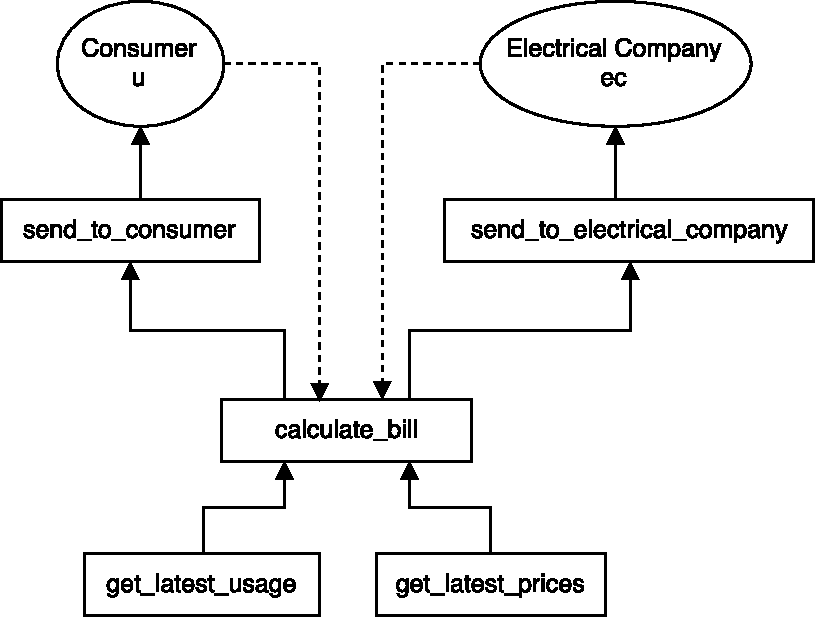
\includegraphics[scale=0.8]{figures/dlm_calculate_bill}
  \caption{Information flow graph for \dlmc{calculate_bill}}
  \label{example:graph:calculate_bill}
\end{figure}

\subsection{Password checker}\label{example:sec:check_password}
A more general example is a simple password checker (see \cref{example:code:check_password} and \cref{example:graph:check_password}), which checks a given username and password combination and checks it against the user database, giving a response to the user whether it was correct or not.
Here we have three auxiliary functions: \dlmc{get_login}, \dlmc{get_users}, and \dlmc{send_response} -- they represent the two inputs needed, as well as the output to be given.

\begin{lstlisting}[float, style=dlmc, numbers=left, caption={Password checker example}, label=example:code:check_password]
#include <stdbool.h>
#include <string.h>

typedef struct user_info {
  char username[20];
  char password[20];
} user_info;

user_info get_login();
user_info *get_users();
void send_response(bool is_match);

bool check_password(char *username,
    char *password) {
  int user_count = 100;
  user_info *users = get_users();
  int i = 0;
  bool match = false;

  while (i < user_count) {
    if (!strcmp(users[i].username, username) &&
        !strcmp(users[i].password, password)) {
      match = true;
    }
    i = i + 1;
  }

  return match;
}

int main(int argc, char **argv) {
  user_info login = get_login();
  bool is_match = check_password(login.username,
      login.password);
  send_response(is_match);
}
\end{lstlisting}

\begin{figure}
  \centering
  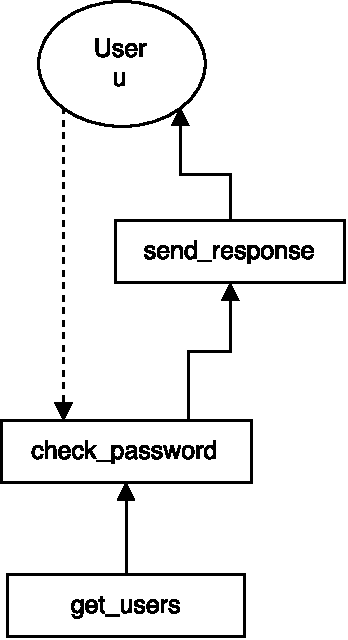
\includegraphics[scale=0.8]{figures/dlm_check_password}
  \caption{Information flow graph for \dlmc{check_password}}
  \label{example:graph:check_password}
\end{figure}
